\section{FPGA vendor dependent protocols}
\label{sec:survey_vendor}
The first protocols to look at, are these delivered by the FPGA vendors. Unfortunately this introduces some complications because the protocol has to function on every FPGA, whatever vendor these are from. Vendors often offer IP-Cores which are only compatible with their specific FPGA's. This could have several reasons like optimization of the hardware structure for certain models, which only the manufacturer knows of course, and which specific parts are included as a hardcore instead of a softcore. Also lots of effort and man hours went into the development of these IP-cores which makes it understandable they are vendor dependent. Nonetheless we will look at these protocols because it is important and interesting to know what the vendors have to offer.

\subsection[Xilinx Aurora]{Xilinx Aurora}
Xilinx Aurora is an existing communication protocol which is as indicated developed by Xilinx and only applicable for Xilinx FPGA's~\cite{Aurora_64B66B_MainPage}. Aurora is designed to ease the implementation of multi-gigabit transceivers in a project and besides that provides a light-weight user interface on top of which designers have the possibility to build a serial link. It is very useful in situations where serial point-to-point connectivity is required like chip-to-chip links.\\
The protocol comes in multiple variants, one of them makes use of the older 8b/10b encoding~\cite{Aurora_8B10B_MainPage} and the other makes use of 64b/66b encoding. This section will be primarily focused on the 64b/66b variant from which a complete IP Product Guide is available~\cite{Aurora_64B66B_IpCore}.\\

The Aurora protocol has a very high throughput that can vary from 0,5 Gbps to over 400 Gbps depending on the amount of available transceivers and their maximum speed. Data can be transferred in simplex or full-duplex mode. Figure~\ref{fig:Aurora_BlockDiagram} shows a block diagram of the protocol~\cite{Aurora_64B66B_IpCore}.
\begin{figure}[ht]
	\centering
	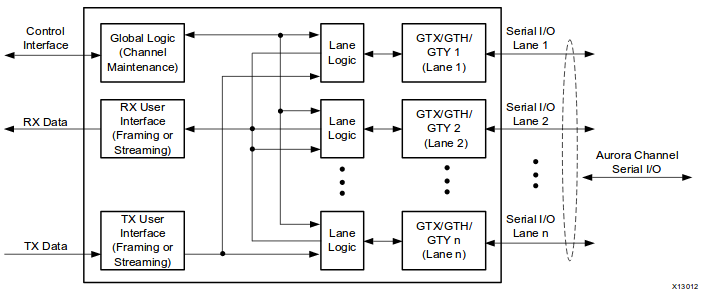
\includegraphics[width=0.77\textwidth]{AuroraBD.png}	
	\caption{The Aurora block diagram.}
	\label{fig:Aurora_BlockDiagram}
\end{figure} 

Every lane contains a separate logic lane where encoding, decoding and error detection happens. The global logic monitors all lane logic modules and is responsible for channel bonding. 
Aurora is also capable of CRC encoding/decoding and flow control.

The CRC32 will be calculated for each individual lane on the valid bytes to be transmitted. There are different variants of flow control to choose from. User flow control (UFC) for example allows the applications to send high-priority messages to each other while native flow control (NFC) allows receivers to regulate the speed at which data will be received. Immediate mode makes it possible to insert idle codes within data frames while completion modes inserts idle codes between complete data frames.
%\begin{figure}[ht]
%	\centering
%	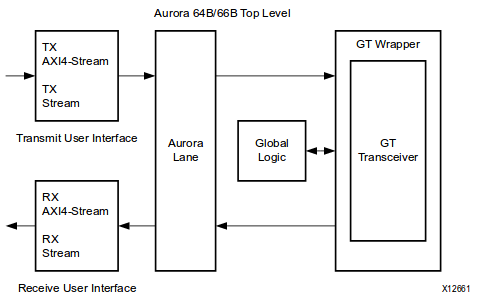
\includegraphics[width=0.7\textwidth]{AuroraTL.png}	
%	\caption{The Aurora Top-Level Architecture. \cite{Aurora64}}
%\end{figure} 

\subsection[Altera/IntelFPGA Serial LITE]{Altera/IntelFPGA Serial LITE}
Altera/IntelFPGA has it's own serial streaming protocol~\cite{SerialLiteIII_MainPage} SerialLite is meant for high bandwidth chip-to-chip, board-to-board and backplane communications. The protocol comes in two variants. The older SerialLite II and the newer SerialLite III. This section will focus on the newer variant of the protocol.

SerialLite can be run in two modes. The continuous and burst mode which both are useful for different applications. In the first mode data will be continuously transmitted without gasps. This is useful when a simple high bandwidth interface is required. The second mode will transmit the data is bursts across the interface. Very useful for applications which send a lot of data at certain moments. Like for example raw digital video content where lines of the display raster can be sent in bursts.

The protocol can be used in simplex and duplex mode which is very useful when needed. Speeds up to 28 Gbps can be reached which is of course very dependent on the transceivers connected to the specific FPGA. Channel bonding with up te 24 lanes is supported which results in possible bandwidth to over 300 Gbps. Transmitted data will be encoded by 64b/67b. All data will also contain CRC-32 error correction.

\begin{figure}[ht]
	\centering
	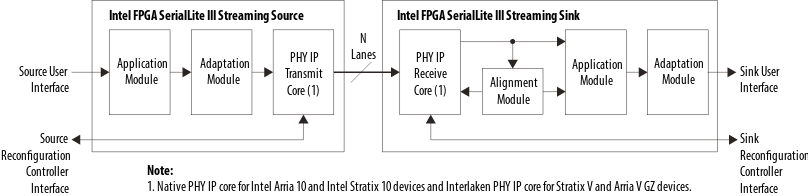
\includegraphics[width=1\textwidth]{SerialLiteIII.png}	
	\caption{The SerialLite III block diagram (Simplex mode).}
	\label{fig:SerialLiteIII_Block}
\end{figure}

In Figure~\ref{fig:SerialLiteIII_Block} the block diagram of the protocol in simplex mode is shown~\cite{SerialLiteIII_IpCore}. The documentation also advertises with low overhead and point-to-point transfer latency. To save soft logic resources it is possible to make use of the hardened Native or Interlaken PHY IP core depending on the model used. The mentioned Interlaken protocol will be discussed in the next section.

\subsection{Microsemi LiteFast}
Microsemi has also developed it's own serial point-to-point link. It is intended as a low-cost, scalable, light weight and high-speed solution. It also provides built-in flow control and in case no data is transmitted link activity will be maintained. 

The protocol includes data framing and in case no data is available idle frames will be transmitted. The data payload will be covered by a CRC-32 packet included at the data frame end. Channel bonding is added as an optional feature and the user can choose between 1, 2 or 4 lanes per SerDes. This supports speeds varying from 4 up to 10 Gbps in case 4 lanes are used. In case multiple lanes are used, the ability to align these is included. Unfortunately the protocol still uses 8b/10b encoding which offers quite the overhead compared to the newer ways of encoding. 
A quick overview of the interface can be seen in Figure~\ref{fig:LiteFast_Block}~\cite{LiteFast_IpCore}.

\begin{figure}[ht]
	\centering
	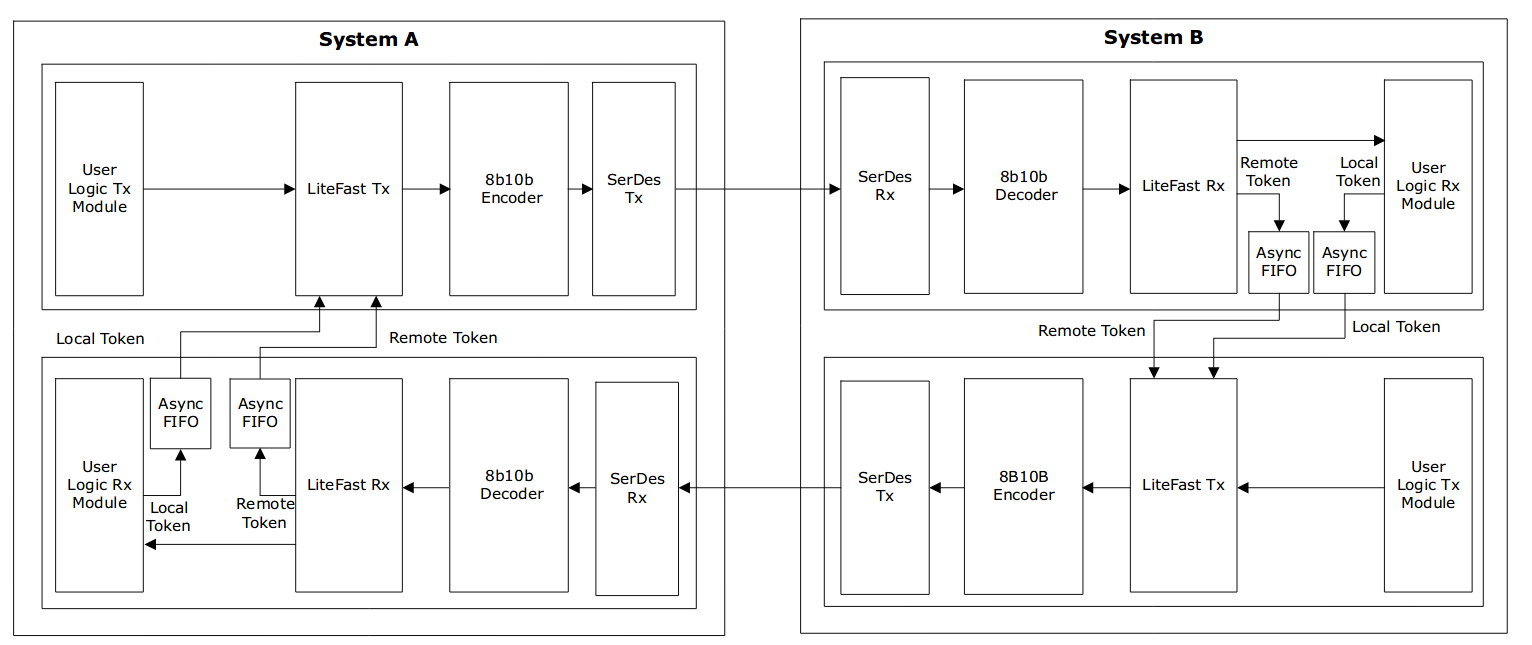
\includegraphics[width=1\textwidth]{LiteFast.png}	
	\caption{The LiteFast block diagram (Single Lane).}
	\label{fig:LiteFast_Block}
\end{figure}

\subsection{Conclusion}
To conclude this section, a bullet point overview of the protocols is added. This will mention the features of both vendor dependent protocols and compare them with each other.\\
\begin{itemize}
	\item Both protocols offer line rates which will push the transceivers to their limits. Aurora mentions about 26 Gbps and Serial Lite III about 28 Gbps per transceiver
	\item Aurora features flow control while Serial Lite III is not clear on this. (In contrast Serial Lite II does support flow control)
	\item Both offer CRC-32 error correction, FEC is not mentioned in the documentations
	\item Aurora uses 64b/66b encoding while Serial Lite III implements 64b/67b line encoding
	\item Both offer excellent channel bonding up to 16 (Aurora) or 24 (Serial Lite) channels which results in speeds to over 300 Gbps \newline
\end{itemize}
\newpage 